%! Author = christophherb


\documentclass[a4paper, 12pt]{article}
%TC:incbib

%%%%%%%% CREATE DOCUMENT STRUCTURE %%%%%%%%
%% Language and font encodings
\renewcommand*{\familydefault}{\sfdefault}
\usepackage[ngerman]{babel}
\usepackage[utf8]{inputenc}
\usepackage[T1]{fontenc}
\usepackage{microtype}% verbesserter Randausgleichjk
\usepackage[scaled]{uarial}
%\usepackage{subfig}

%% Sets page size and margins
\usepackage[a4paper,top=3cm,bottom=2cm,left=2cm,right=2cm,marginparwidth=1.75cm]{geometry}

%% Packages
\usepackage{amsmath}
\usepackage{graphicx}
\usepackage[colorlinks=true, allcolors=black]{hyperref}
\usepackage{caption}
\usepackage{subcaption}
\usepackage{sectsty}
\usepackage{apacite}
\usepackage{float}
\usepackage{titling}
\usepackage{blindtext}
\usepackage[square,sort,comma,numbers]{natbib}
\usepackage[colorinlistoftodos]{todonotes}
\usepackage{xcolor}
\definecolor{darkgreen}{rgb}{0.0, 0.4, 0.0}
\definecolor{LightGray}{gray}{0.8}
\usepackage{verbatim}
\usepackage{booktabs}
\usepackage{longtable}
\usepackage{pdfpages}
\usepackage[outputdir=build]{minted}

\setcounter{secnumdepth}{4}

%%%%%%%% Functions %%%%%%%%
%% Count Characters
\newcommand{\charactercount}[1]{
    \immediate\write18{
        expr `texcount -1 -sum -merge #1.tex` + `texcount -1 -sum -merge -char #1.tex` - 1
        > build/.chars.txt
    } 
    \input{build/.chars.txt}
}

%% Count Words
\newcommand{\quickwordcount}[1]{%
    \immediate\write18{
      texcount -1 -sum -merge -q #1.tex > build/.#1-words.sum 
    }
    \input{build/.#1-words.sum}%
}


%%%%%%%% Variables %%%%%%%%
\newcommand{\HRule}{\rule{\linewidth}{0.5mm}} 							% horizontal line and its thickness


%%%%%%%% DOCUMENT %%%%%%%%
%%%% Title Page
\begin{document}
    \begin{titlepage}
        \center
        %\vspace*{2.0cm}
        \includegraphics[width=0.45\textwidth]{../images/hsa_logo}\\[0.5cm] 	% University logo
        \includegraphics[width=0.3\textwidth]{../images/logo}\\[1.5cm] 	% University logo

        \HRule \\[0.2cm]
        {
          \huge \bfseries todo\\
          \large Dokumentation der Anwendung\\[0.5cm]
          \large Full-Stack-Webanwendungen\\
          \large Sommersemester 2023
        }\\[0.2cm]								% Assignment
        \HRule \\[2cm]

        \begin{flushleft}
          \large
          Lucas Schiessl\\
          lucas.schiessl@hs-augsburg.de\\
          Informatik\\[0.5cm]

          Hannes Ziereis\\
          hannes.ziereis@hs-augsburg.de\\
          Informatik\\[0.5cm]

          Christoph Herb\\
          christoph.herb@hs-augsburg.de\\
          Informatik\\[2cm]

          \charactercount{main} Zeichen (mit Leerzeichen)\\
        \end{flushleft}
        %{\large \today}\\[5cm]
        \vfill
    \end{titlepage}

%%\begin{abstract}
%%Your abstract.
%%\end{abstract}
\tableofcontents

%%%% SECTIONS
%% Section 1
\newpage
    \section{Allgemein}
    \subsection{Beschreibung}
    Ziel dieser Arbeit war es, eine Applikation für das Verwalten von Todos zu implementieren. Der Nutzer soll sich in der Webanwendung zuerst 
    registrieren und dann über einen Login anmelden können. Nach der Anmeldung kann der User dann neue Tasks hinzufügen, vorhandene editieren
    und lösche sowie sich eine Gesamtübersicht aller geplanten Tasks im Kalender anzeigen lassen. Die Daten des Users können zudem
    in einem eigenen Fenster bearbeitet werden. Weitere Informationen dazu sind im Frontend, Backend und Datenbank-Teil dieser Anwendung
    beschrieben. Zum Starten und Betreiben (Default Credentials der User, Datenbank-Zugang) der Anwendung sind weitere Informationen in der {\it README.md} 
    des Projekts enthalten.

    \subsection{Organisation}
    Für die Organisation und Verwaltung des Quellcodes wurde GitLab benutzt. Dieses bietet neben der Quellcodeverwaltung auch die 
    Möglichkeit noch offene Aufgaben zu verwalten (Issues), CI/CD-Pipelines zu erstellen (CI/CD) und Container-Images zu speichern (Packages \& Registry).
    Zu Beginn des Projektes wurden Issues für die einzelnen Kernfunktionen erstellt und priorisiert. 
    Im Laufe des Projektes wurden dann für Fehler und zusätzliche Funktionen weitere Issues hinzugefügt und nacheinander abgearbeitet.
    So war zu jeder Zeit sichtbar, welche Aufgaben bereits abgearbeitet wurden und welche noch offen sind. 
    Eine Übersicht aller Issues und deren zugeteilte Person findet man im Anhang~\ref{issues}.

    \subsection{Aufbau}

    \begin{figure}[H]
        \center\includegraphics[width=0.6\textwidth]{../images/architecture.drawio}
        \caption{Architektur der deployten Anwendung}\label{fig:figure}
    \end{figure}

    \section{Frontend}
    \subsection{Design}

    \begin{figure}[H]
        \center\includegraphics[width=0.7\textwidth]{../images/figma/login}
        \caption{Figma Design des Logins}\label{fig:figure}
    \end{figure}

    \begin{figure}[H]
        \center\includegraphics[width=0.7\textwidth]{../images/figma/register}
        \caption{Figma Design des Registrierungsformulars}\label{fig:figure}
    \end{figure}

    \begin{figure}[H]
        \center\includegraphics[width=0.7\textwidth]{../images/figma/main}
        \caption{Figma Design der Hauptseite}\label{fig:figure}
    \end{figure}

    \subsection{Funktionen}
    Das Frontend kann untergliedert werden in folgende Teilbereiche:

    \begin{itemize}
        \item Login und Registrierung
        \item Taskübersicht
        \item Navigationsleiste
    \end{itemize}

    Für das Login wurde mit Pinia ein Auth Store und ein User Store angelegt. Der Auth Store wird dabei für Login und
    Logout, sowie das Speichern und Refreshen des Authentication Tokens verwendet. Der User Store wird verwendet um den
    aktuellen Benutzer abzufragen, einen neuen Nutzer anzulegen oder zu updaten.
    
    Über die Login Seite hat der Nutzer die Möglichkeit sich in der Anwendung anzumelden. Zudem kann durch Klick auf
    {\it Registration} ein neuer Nutzer angelegt werden. Ist der Nutzer nicht authentifiziert wird er immer zur Login
    Seite redirected. Das Passwortfeld in der Login- und Registrierungsmaske wurde um einen Button ergänzt, der es dem
    Nutzer erlaubt das Passwort im Klartext anzuzeigen, falls gewünscht. Ist der Login erfolgreich, wird der Nutzer auf
    die Home View weitergleitet und ein Authentication Token im lokal Storage gespeichert.

    Ein neuer Benutzer kann über die Registrierungsseite angelegt werden. Dabei müssen Vor- und Nachname, Email Adresse
    und Passwort angegeben, sowie das Passwort bestätigt werden. Ist ein Feld leer oder nicht korrekt ausgefüllt wird
    eine entsprechende Fehlermeldung darunter angezeigt. Wird der Nutzer erfolgreich angelegt, wird der Nutzer auf eine
    Registration Success Seite weitergeleitet. Anschließend kann man sich einloggen.

    Auf der Main Page befindet sich links die Navigationsleiste und rechts die Tasks des aktuell eingeloggten Nutzers.
    Auf der Navigationsleiste kann der Nutzer zwischen einer Listen und einer Kalender Ansicht der Tasks wählen. Zudem
    können die Tasks nach den ihnen zugewiesenen Tags gefiltert werden. Am unteren Rand der Navbar wird der Name, die
    Email Adresse und die Initialen des aktuell eingeloggten Nutzers angezeigt. Die Initialen könnten in einer
    zukünftigen Version durch ein Profilbild ersetzt werden. Über dieser Anzeige hat der Nutzer die Möglichkeit sich
    wieder auszuloggen, oder die Einstellungen zu ändern.

    Die Settings Seite bietet dem Benutzer die Möglichkeit seinen Namen und sein Passwort, sowie die Sprache der App zu
    ändern. Die Texte der App wurden mit dem i18n Plugin für Vue implementiert, so dass zusätzliche Sprachen einfach
    hinzugefügt werden können. Aktuell unterstützt werden Deutsch und Englisch.

    Auf der rechten Seite der Main Page befinden sich die Tasks in einer Liste. In der Liste werden der Titel und falls
    vorhanden eine verkürzte Beschreibung, der Tag und das Fälligkeitsdatum der Aufgabe angezeigt. Klickt man auf einen
    Task, öffnet sich eine Detail Ansicht als Modal Fenster. In dieser werden alle Attribute des Tasks angezeigt. Zudem
    hat der Nutzer die Möglichkeit den Task zu löschen, oder zu bearbeiten.

    Wenn das Modal während des Bearbeiten geschlossen wird, entweder durch den X-Button oder durch klicken außerhalb des
    Modals, bleiben die vorgenommen Änderungen erhalten und können bei erneutem öffnen des Tasks weiter bearbeitet
    werden. Die Persistierung der Änderungen findet im localStorage des Browsers statt.

    Ein neuer Task kann durch das unterste Item der Task Liste angelegt werden. Dafür wird mindestens ein Titel
    benötigt, alle anderen Attribute können durch das Ausklappen des Items eingetragen werden.

    Klickt man auf {\it Scheduled Tasks} wird die Task Liste durch eine Kalender Ansicht ersetzt. Hier werden allerdings
    nur die Tasks angezeigt, die ein Fälligkeitsdatum als Attribut besitzen. Falls der Task zudem einen zugewiesenen Tag
    hat, wird der Task in der entsprechenden Farbe angezeigt. Auch in der Kalender Ansicht kann durch Klick auf den Task
    das Task Detail Modal geöffnet werden.


    \section{Backend}
    \subsection{Funktionen}

    Das Backend ist in TypeScript implementiert und verwendet das Prisma ORM für den Datenbankzugriff.

    Im Backend gibt es verschiedene Service-Module wie user.service.ts und task.service.ts, die die Logik für die
    Benutzerverwaltung und die Aufgabenverwaltung enthalten. Der user.service.ts ermöglicht das Erstellen, Lesen,
    Aktualisieren und Löschen von Benutzerdaten. Der task.service.ts ermöglicht das Erstellen, Lesen, Aktualisieren und
    Löschen von Aufgaben. Beide Services arbeiten eng mit der Prisma-Datenbank zusammen, um die Daten persistent zu
    speichern.

    Die Routenmodule wie user.route.ts und task.route.ts definieren die API-Endpunkte für die Benutzerverwaltung und die
    Aufgabenverwaltung. Diese Endpunkte sind durch Sicherheitsmechanismen wie JWT-Authentifizierung geschützt. Die
    Routenmodule rufen die entsprechenden Funktionen aus den Service-Modulen auf und geben die Ergebnisse als JSON an die
    Client-Anwendung zurück.

    Das Backend verwendet auch verschiedene Hilfsmodule wie helpers.ts, um Validierungen und andere allgemeine Aufgaben zu
    unterstützen. Es gibt auch Exception-Module, die spezifische Fehlerklassen wie NotFoundError oder ValidationError
    enthalten, um Fehler in der API-Behandlung zu verwalten und entsprechende HTTP-Statuscodes und Fehlerantworten zu
    generieren. Die komplette API des Backends wurde außerdem mithilfe von Swagger dokumentiert und kann nach dem Start
    im DEV Modus über die URL http://localhost:3000/api-docs aufgerufen werden. Außerdem wurde die Dokumentation als
    PDF exportiert und kann im Anhang~\ref{api} dieser Dokumentation gefunden werden.

    \subsection{Tests}

    Die Verwendung von Cucumber.js ermöglicht es, Tests in einer natürlichen Sprache zu schreiben, die für alle Projektbeteiligten leicht
    verständlich ist. Die Testszenarien werden in sogenannten Feature-Dateien definiert, während die Schritte in den Step-Definitionen
    implementiert werden.

    Die Feature-Datei (task.feature) enthält beschreibende Szenarien, die die verschiedenen Anwendungsfälle für Tasks abdecken. Jedes Szenario
    besteht aus einem Titel, einer Beschreibung und einer Liste von Schritten. Die Schritte beschreiben
    den Zustand, die Aktion und die erwartete Überprüfung für jeden Schritt.

    Die Step-Definitionen (api\_steps.ts) enthalten die Implementierung der Schritte aus den Feature-Dateien. Hier wird die Testlogik für jeden
    Schritt definiert, einschließlich der Interaktion mit dem zu testenden System (z.B. HTTP-Anfragen senden) und der Überprüfung des erwarteten
    Verhaltens (z. B. Überprüfen des Statuscodes und des Antwortformats).

    Die ApiSteps-Klasse enthält Methoden, die mit den Annotationen @given, @when und @then markiert sind, um die entsprechenden Schritte
    abzudecken. In den Methoden werden die Aktionen und Überprüfungen ausgeführt, um den Testfall zu validieren.

    Die Task-Tests folgen einem BDD-Ansatz (Behavior-Driven Development), bei dem die Testszenarien aus der Sicht des Endbenutzers formuliert
    werden. Die Szenarien beschreiben typische Abläufe wie das Erstellen, Aktualisieren, Löschen und Abrufen von Tasks. Die Step-Definitionen
    stellen sicher, dass diese Szenarien automatisch getestet werden können.

    In {\tt user.feature} und {\tt auth.feature} sind, ähnlich wie in {\tt task.feature} die Tests für den User- und Authentifizierungsteil des Backends definiert.

    Während der Ausführung der Tests wird Cucumber.js die Feature-Dateien und die zugehörigen Step-Definitionen analysieren. Für jeden Schritt
    in einem Szenario wird die entsprechende Methode in den Step-Definitionen aufgerufen, um die Aktion auszuführen und die Überprüfungen
    durchzuführen. Die Testergebnisse werden dann zusammengefasst und ausgegeben, um zu zeigen, welche Szenarien erfolgreich waren und welche
    fehlgeschlagen sind. Die Tests können mit folgendem Befehl gestartet werden.

    \begin{minted}[
    baselinestretch=1.2,
    fontsize=\footnotesize,
    ]{bash}
# Start dependencies
docker-compose up -d

# Execute tests
yarn test:integration
    \end{minted}

    \begin{figure}[H]
    \begin{minted}
    [
    baselinestretch=1.2,
    fontsize=\footnotesize,
    ]{cucumber}
@auth
Feature: Authentication
  Login user, verify user, refresh token

  Scenario: Login user (correct email/password)
    Given the Content-Type is 'application/json'
    When I send a POST request to "http://localhost:8000/api/v1/auth/login" with json:
      """
        {
          "email": "admin@todo.com",
          "password": "admin"
        }
      """
    Then the response code should be 200
    And the response body should be json:
      """
        {
          "tokenType": "Bearer",
          "accessToken": String
        }
      """
    \end{minted}
    \caption{Beispiel eines Cucumber Integration Tests}\label{fig:figure}
    \end{figure}


    \section{Datenbank}
    \subsection{Postgresql}
    Als Datenbank wurde eine Postgresql DB verwendet. Da für den Datenbankzugriff Prisma ORM verwendet wurde, sind die Tabellen
    in der backend/prisma/schema.prisma Datei definiert. Um Testdaten in die Datenbank zu schreiben wird die Datei backend/prisma/seed.ts einmalig
    beim Hochfahren der Datenbank ausgeführt. Die Tabellen und ihre Relationen können in der folgenden Grafik eingesehen werden:
    
    \begin{figure}[H]
        \center\includegraphics[width=0.7\textwidth]{../images/database}
        \caption{Datenbank Diagramm}\label{fig:figure}
    \end{figure}

    \subsection{Redis}
    Für die Speicherung der abgelaufenen Token wurde eine Redis Datenbank verwendet. Redis ist eine Key-Value Datenbank, das heißt alle Daten sind als
    Key-Value-Paare in der Datenbank gespeichert. In unserem Use-Case, dem Abspeichern von abgelaufenen Tokens nach dem Logout, wird das Token als
    Key gespeichert. Nach jedem {\it verify} des Tokens wird also zusätzlich abgefragt, ob das Token sich in der Blacklist-Datenbank befindet.
    Redis hat den Vorteil, dass es sehr leichtgewichtig und schnell ist. Zudem hat es die Funktion, dass Values nach einer bestimmten Zeit automatisch
    aus dem Speicher gelöscht werden können. So können in unserem Fall Token, die abgelaufen sind, aus dem Blacklist-Store entfernt werden, wodurch die
    Datenbank nie sehr groß wird und somit Speicherplatz und Latenzzeit eingespart werden kann.

    \newpage
    \section{Quellen}
    \subsection{Code-Teile von Dritten}
    \subsubsection{Frontend}
\begin{itemize}
  \item dockerfile for production: https://medium.com/bb-tutorials-and-thoughts/how-to-serve-vue-js-application-with-nginx-and-docker-d8a872a02ea8
  \item nginx config: https://www.appsyoda.com/blog/deploying-vuejs-app-using-nginx/
  \item combobox styled: https://headlessui.com/react/combobox
\end{itemize}

    \subsubsection{Backend}

\begin{itemize}
  \item https://github.com/domideimel/error-middleware  (not maintained anymore)
  \item help from here: https://www.elliotdenolf.com/blog/cucumberjs-with-typescript
  \item redis singleton client: https://stackoverflow.com/questions/54240635/how-to-make-express-js-app-connect-redis-only-1-time-when-the-app-start-without
  \item how to emulate object enums: https://stackoverflow.com/questions/41179474/use-object-literal-as-typescript-enum-values
  \item prisma middleware for hashing passwords: https://stackoverflow.com/questions/69233726/cannot-hash-the-users-password-with-prisma-middleware-in-nestjs-on-create-user
\end{itemize}

    \newpage
    \subsection{Bibliotheken}
    \subsubsection{Frontend}

    \begin{minted}[frame=none,
               framesep=3mm,
               linenos=true,
               xleftmargin=21pt,
               tabsize=4]{js}
"dependencies": {
  "@headlessui/tailwindcss": "^0.1.3",
  "@headlessui/vue": "^1.7.14",
  "@heroicons/vue": "^2.0.17",
  "@preline/overlay": "^1.4.0",
  "@vuepic/vue-datepicker": "^5.2.0",
  "@vueuse/core": "^10.1.2",
  "autoprefixer": "^10.4.14",
  "axios": "^1.3.4",
  "pinia": "^2.0.33",
  "postcss": "^8.4.21",
  "preline": "^1.7.0",
  "storejs": "^2.0.5",
  "tailwindcss": "^3.2.7",
  "vue": "^3.2.47",
  "vue-final-modal": "^4.4.2",
  "vue-i18n": "9",
  "vue-router": "^4.1.6",
  "vue-simple-calendar": "^6.3.1"
},
"devDependencies": {
  "@rushstack/eslint-patch": "^1.2.0",
  "@types/jsdom": "^21.1.0",
  "@types/node": "^18.14.2",
  "@vitejs/plugin-vue": "^4.0.0",
  "@vue/eslint-config-typescript": "^11.0.2",
  "@vue/test-utils": "^2.3.0",
  "@vue/tsconfig": "^0.1.3",
  "autoprefixer": "^10.4.14",
  "cypress": "^12.7.0",
  "eslint": "^8.34.0",
  "eslint-plugin-cypress": "^2.12.1",
  "eslint-plugin-vue": "^9.9.0",
  "jsdom": "^21.1.0",
  "npm-run-all": "^4.1.5",
  "postcss": "^8.4.21",
  "start-server-and-test": "^2.0.0",
  "tailwindcss": "^3.2.7",
  "typescript": "~4.8.4",
  "vite": "^4.1.4",
  "vitest": "^0.29.1",
  "vue-tsc": "^1.2.0"
}
    \end{minted}
    \subsubsection{Backend}
    \begin{minted}[frame=none,
               framesep=3mm,
               linenos=true,
               xleftmargin=21pt,
               tabsize=4]{js}
"dependencies": {
  "@prisma/client": "^4.11.0",
  "class-validator": "^0.14.0",
  "cookie-parser": "^1.4.6",
  "datejs": "^1.0.0-rc3",
  "dayjs": "^1.11.8",
  "dotenv-cli": "^7.1.0",
  "express": "^4.18.2",
  "express-actuator": "^1.8.4",
  "express-async-handler": "^1.2.0",
  "express-jsdoc-swagger": "^1.8.0",
  "express-promise-router": "^4.1.1",
  "jsonwebtoken": "^9.0.0",
  "ms": "^2.1.3",
  "prisma": "^4.11.0",
  "redis": "^4.6.6",
  "tslog": "^4.8.2"
},
"devDependencies": {
  "@cucumber/cucumber": "^9.0.1",
  "@types/chai": "^4.3.5",
  "@types/chai-json-pattern": "^1.1.0",
  "@types/cookie-parser": "^1.4.3",
  "@types/cucumber": "^7.0.0",
  "@types/datejs": "^0.0.33",
  "@types/express": "^4.17.17",
  "@types/express-actuator": "^1.8.0",
  "@types/jsonwebtoken": "^9.0.1",
  "@types/ms": "^0.7.31",
  "@types/node": "^18.15.5",
  "@types/swagger-ui-express": "^4.1.3",
  "axios": "^1.3.4",
  "chai": "^4.3.7",
  "chai-json-pattern": "^1.1.0",
  "cucumber-html-reporter": "^6.0.0",
  "cucumber-tsflow": "^4.0.0-rc.11",
  "nodemon": "^2.0.21",
  "ts-node": "^10.9.1",
  "typescript": "^5.0.2"
}
    \end{minted}

    \newpage
    \section{Anhang}
    \subsection{GitLab Issues}
    \begin{longtable}{ll}
\label{GitLab Issues} \\
\toprule
Title & Assignee \\
\midrule
\endfirsthead
\toprule
Title & Assignee \\
\midrule
\endhead
\midrule
\multicolumn{2}{r}{Continued on next page} \\
\midrule
\endfoot
\bottomrule
\endlastfoot
FE Install Tailwindcss & Lucas Schießl \\
BE Create blueprint for backend & Christoph Herb \\
BE Add postgresql & Lucas Schießl \\
BE Add refresh endpoint & Christoph Herb \\
BE Add getting started documentation & Christoph Herb \\
DOC Create documentation & NaN \\
FE Create Figma Design & Christoph Herb \\
BE Create Database model & Hannes Ziereis \\
BE Implement swagger docs or create REST-API diagram manually & Lucas Schießl \\
FE Implement basic design & Lucas Schießl \\
FE First interaction with BE & Christoph Herb \\
FE Implement authentication with BE & Lucas Schießl \\
FE Cleanup frontend & Christoph Herb \\
FE Implement Nav Bar and design Login Form & Lucas Schießl \\
BE Endpoints for tasks & Hannes Ziereis \\
FE Interaction with tasks & Hannes Ziereis \\
BE Implement better logger & Christoph Herb \\
BE Hash password before saving into DB & Christoph Herb \\
FE Implement login in frontend & Lucas Schießl \\
FE style login form & Lucas Schießl \\
FE create Registration Form & Lucas Schießl \\
BE Add logout endpoint & Christoph Herb \\
FE Add error handling to login and registration form & Lucas Schießl \\
BE Fix tasks endpoint, swagger docs and cucumber tests & Christoph Herb \\
BE, FE Add docker support & Christoph Herb \\
FE Call Logout and refresh endpoints from frontend & Lucas Schießl \\
BE Fix bugs in backend & Christoph Herb \\
DOC Add postman collection & Christoph Herb \\
FE Add more functionality to task bar & Lucas Schießl \\
FE Add functionality to settings page & Lucas Schießl \\
FE Refactoring & Lucas Schießl \\
FE Refresh does not work as expected & Lucas Schießl \\
BE, FE Fix docker prod environment & Christoph Herb \\
BE Error messages for frontend & Christoph Herb \\
BE Sorting of tasks with date & Christoph Herb \\
BE Add filtering for categories & Christoph Herb \\
FE Add support for multiple languages & Lucas Schießl \\
FE Show taskdetails in task list & Hannes Ziereis \\
FE Refactor AppTask into its components & Hannes Ziereis \\
BE Move password hashing to postgres & Christoph Herb \\
FE Cleanup & Christoph Herb \\
BE Generate secrets instead of hard coding & Christoph Herb \\
BE Add optional Tags to Tasks & Lucas Schießl \\
FE Fix token refresh endless loop & Christoph Herb \\
FE Add calendar for scheduled tasks & Christoph Herb \\
FE Show Tag in overview and details modal & NaN \\
FE BUG - Modals opens two times & Christoph Herb \\
FE Detailed View - Done status doesn't update & Christoph Herb \\
FE Fix styling of task list & Christoph Herb \\
FE  Edit Task in Detail modal & Hannes Ziereis \\
FE Improve modal & Christoph Herb \\
\end{longtable}

    \label{issues}

    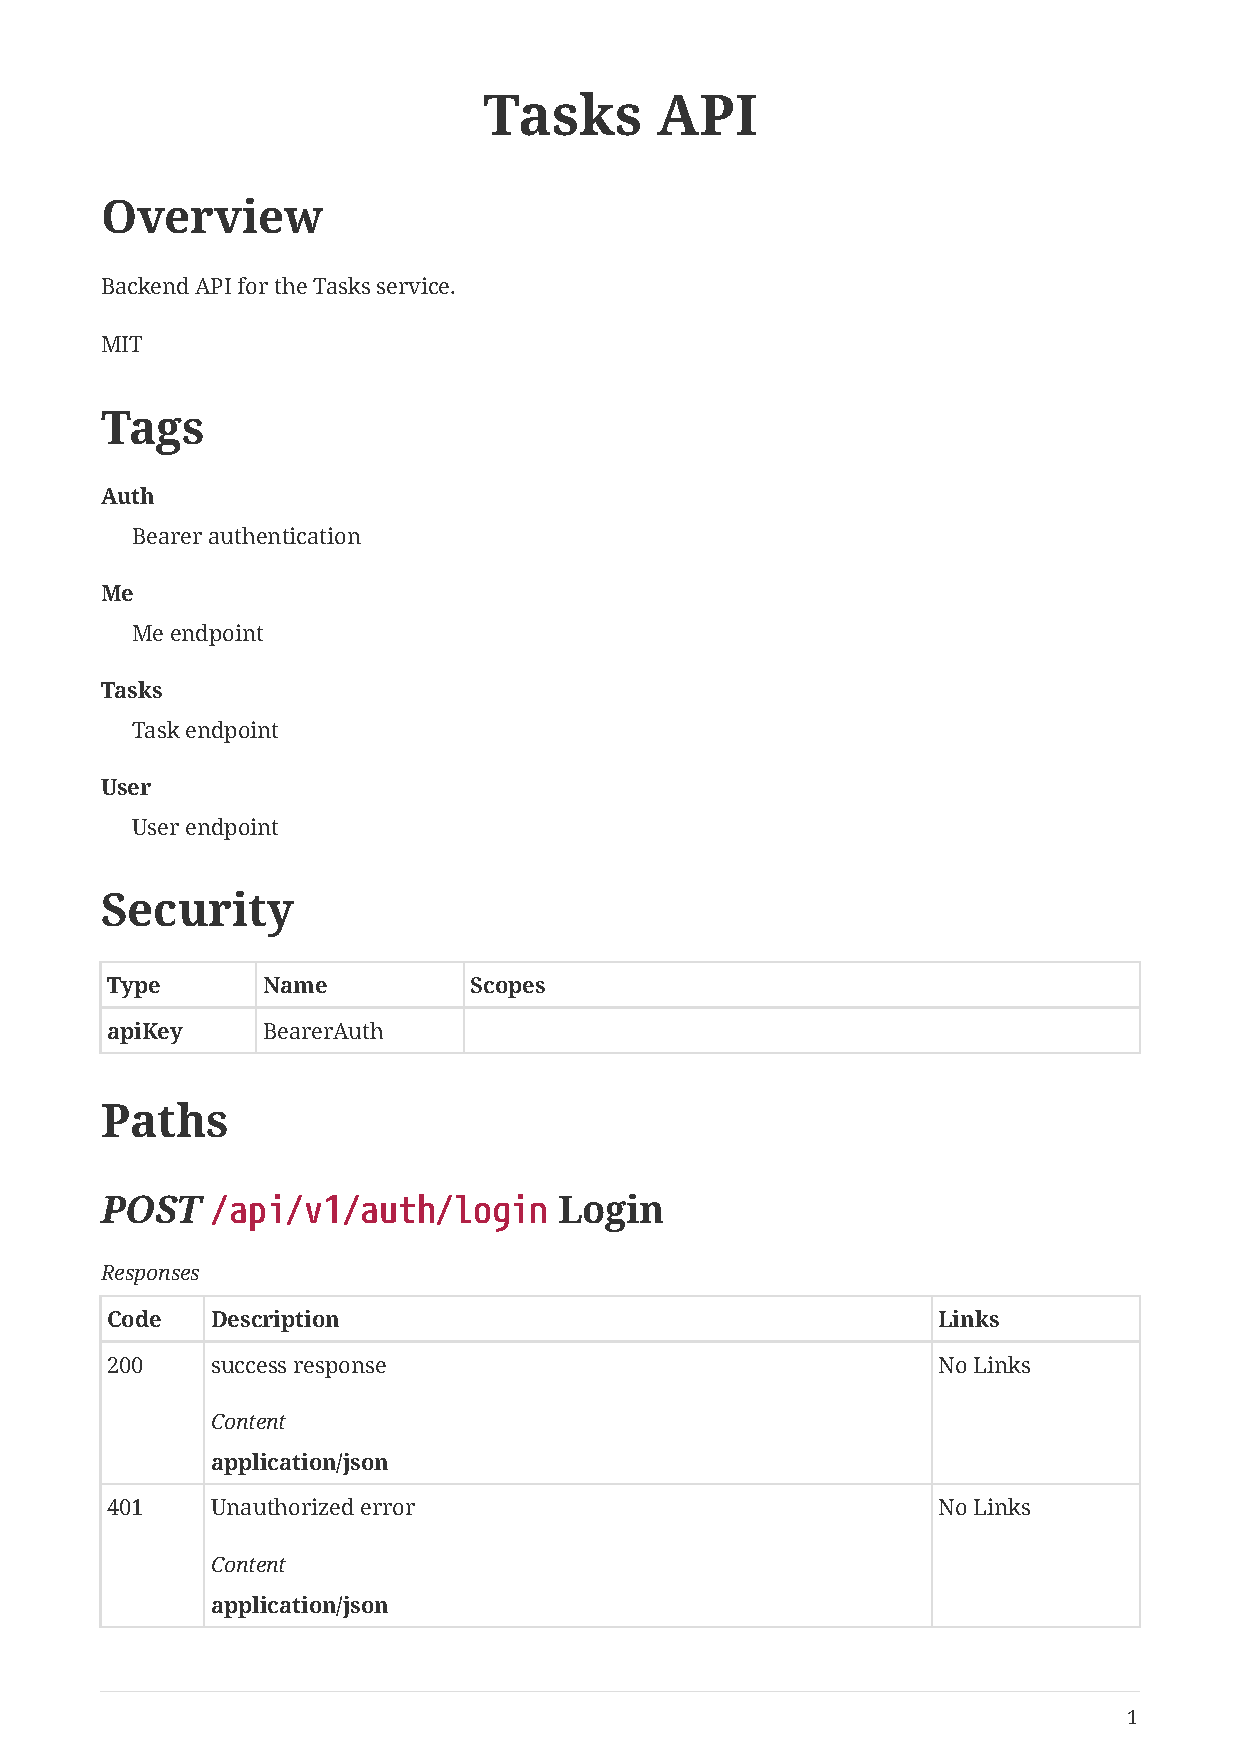
\includepdf[pages=1,scale=.85,pagecommand={\subsection{API Dokumentation}}]{../appendix/swagger_docs.pdf}
    \includepdf[pages=2-,scale=.85,pagecommand={}]{../appendix/swagger_docs.pdf}
    \label{api}


    % \begin{figure}[H]
    %     \includegraphics[width=\textwidth]{images/organigram}
    %     \caption{Organigramm Team Pyramid 2021}\label{fig:figure}
    % \end{figure}

    \newpage

\includepdf[pages=1,pagecommand={\subsection{Erstellungserklärung}}]{../documents/erstellungserklaerung_fullstack_todo_app}

\end{document}
